\documentclass[]{article}
\usepackage{graphicx}
%opening
\title{Physics 117 Lab 1}
\author{Shijia (Scarlett) Yu \\Lab Partner: Edward Polanco\\Prof. Musumeci, TA: Albert Brown}
\date{January 11, 2017}

\begin{document}
	\maketitle
\subsection* {Beginning exercises:}
	\paragraph { (a)} %\mbox{}\\
		We set the DC power supply to 5V to get voltage readings on the lab-bench voltmeter, a DVM, and the oscilloscope. The lab-bench multimeter and the DVM both gave similar reading, but the scope's reading is a little off. So, in terms of precision, it's better to use DVM or multimeter to measure voltage.
			\begin{center}
			\begin{tabular}{|c|c|}
				\hline
				Equipment & Voltage(V) \\
				\hline
				Lab-bench voltmeter & 5.200\\
				\hline
				DVM &  5.201\\ 
				\hline
				Oscilloscope & 5.250 \\
				\hline
			\end{tabular}
		\end{center}
	\paragraph{ (b)} 
		(1) We cannot directly hook up ammeter to voltage source because Ammeter is made to have a very low resistance (ideally zero). So connecting ammeter with a power source would create a short circuit, burning out the fuse inside the Ammeter. \\
		(2) For a multimer to give us Ohms reading, it must calculate the voltage and current across the element that's connected to it. The multimeter does it by internally setting a potential difference between its postive and negative ends, then measuring the current flowing through, and then calculating resistance using Ohm's Law. So, if you connect the multimeter with Ohms mode to a voltage source, the actual voltage across the element is different than the voltage used by the multimeter in its calculation, but the current is the same. Thus, you'll get a wrong reading of the resistance.
		
	\paragraph{ (c)} 
	In the figure below, 
		\begin{center}
		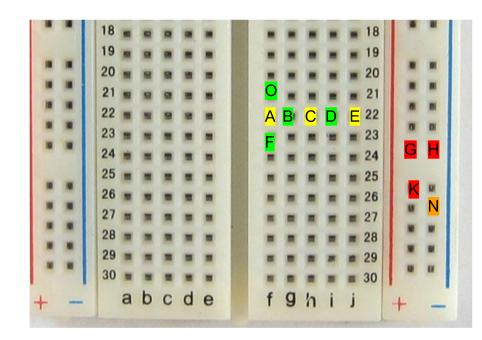
\includegraphics[scale=0.4]{lab1_1}\\
		Figure 1: Busbar connections
		\end{center}
		the busbars: \\
			A,B,C,D,E (horizontal columns) are connected with each other,\\
			AF,AO, or OF (verticle row) not connected with each other, \\
			BO are not connected\\
			GK, HN are connected,\\
			KN are not connected
	\paragraph{ (d)}
	Ohm's Law verification: We used a 2k$\Omega$ resistor, connected in series with the lab-bench ammeter, and in parrallel with the oscilloscope. The ammeter gave the reading in mA, the oscilloscope read the voltage. Using Ohm's Law, the calculated resistance is $R=V/I$. The calculated results are within 5\% relative error, so we confirmed the Ohm's Law. 
	\begin{center}
		\begin{tabular}{|c|c|c|}
			\hline
			Voltage(V) & Current(mA) & Resistance ($\Omega$) \\
			\hline
			5.36& 2.643& 2065\\
			\hline
			6.10 & 2.980& 2047\\ 
			\hline
			6.20 & 3.068& 2026\\
			\hline
		\end{tabular}
		\\Table 1: I,V measurements for Ohm's law verification
	\end{center}
	
\subsection*{ Effects of instruments on your readings}	
	\paragraph{ (e)}
	To measure the internal resistance of an Ammeter, we first used multimeter to measure the resistnace of a resistor (we used a known 2k$\Omega$ resistor). The displayed resistance was 1973$\Omega$. Then we measured the resistance of the resistor plus the ammeter, while they were connected in series. The total resistance was 1978$\Omega$. So, subtracting the two resistances, we got 5$\Omega$ for the ammeter internal resistnace.\\ We usually can't measure the ammemter's resistance with an Ohmmeter, because ammeters are made to have very low resistance. Internal resistance could be 0.1$\Omega$ or 0.0001$\Omega$, which would be too small to be measured by Ohm-meter. In this case, the internal resistance is on the magnitude of ohms, so we can use the Ohm-meter.
	\paragraph{ (f)}
	We used the Ohm-metetor measure the resistance of a resistor on a breadboard to 9.99M $\Omega$. Then, I held my fingers to the two leads of the resistor while I sat on a chair with my feet not on the ground, effectively connecting myself in parralle to the resistor. The Ohm-meter reading dropped to around 0.300 M$\Omega$.\\ When I stood up on my feet, the Ohm-meter reading dropped even lower to 0.956 M$\Omega$. This is becuase I was like a voltage divider, so some of the voltage went through me and the Ohmeter measured the combined resistance of the resistor and me. \\In the case of 10k$\Omega$, holding my fingers to the lead didn't have too impact since humans have significantly higher resistance. 

	\paragraph{ (g)}
	To dissipate 2.5W in a resistor with 5V power, we'll need $I=\frac{P}{V} =\frac{2.5W}{5V} =0.5A$. So the resistance we need is $R=\frac{V}{I}= \frac{5V}{0.5A}=10\Omega\ $. When we applied 5V to a 1/4W 10$\Omega$ resistor, the resistor was burnt.
	
\subsection*{ Testing Ohm's law on lamp}	
	\paragraph{ (h)}
	We took around 15 I-V data points as we incresased the voltage (by decreasing the resistance of potiomenter) until the lamp burnt out. Then we plotted the lamp's I-V curve. 
		\begin{center} 
			$\begin{array}{ | l | l |  }
			\hline
			V (mV) & I (mA) \\ \hline
			0.6 & 5.241 \\ \hline
			1.2 & 7.300   \\ \hline
			1.8 & 9.042 \\ \hline
			2.4 & 10.600\\ \hline
			3 & 11.750 \\ \hline
			3.6 & 13.50 \\ \hline
			4.2 & 14.370 \\ \hline
			5.9 & 17.588 \\ \hline
			7.1& 19.700 \\ \hline
			8.7 & 22.004  \\ \hline
			9.3& 22.880 \\ \hline
			10.8& 24.993 \\ \hline
			11.5& 25.770 \\ \hline
			12.5& 26.542 \\ \hline
			14.1& 28.000 \\ \hline
			\end{array}$\\
			\title{Table 2: Measured I-V data of a lamp}
		\end{center}
		\begin{center} 
			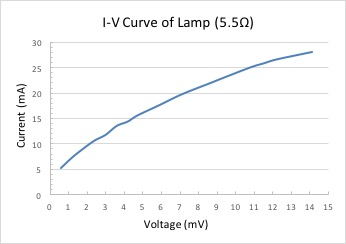
\includegraphics[scale=0.7]{lab1_lampplot}\\			
			Figure 2: I-V curve of the lamp
		\end{center}
	The figure above shows that the curve starts out  linearly increasing, but at higher voltage, it becomes non-ohimc. This is becuase as we put more power to the lamp, the temperature of the lamp got higher, causing the resistance of the lamp to vary. \\
	From the plot, we see the curve from 0V to 4V is pretty linear, so we can say the "resistance" (slope of the line) of the lamp is 5.5$\Omega$ in that region.
	
\subsection*{ Testing Ohm's law with diode}	
	\paragraph{ (i)}
	We conncted the cirucit as below, using a potentiometer with the range of 0.2 $\Omega$ - 103.6 $\Omega$ to vary the voltage going through the diode.
	\begin{center} 
		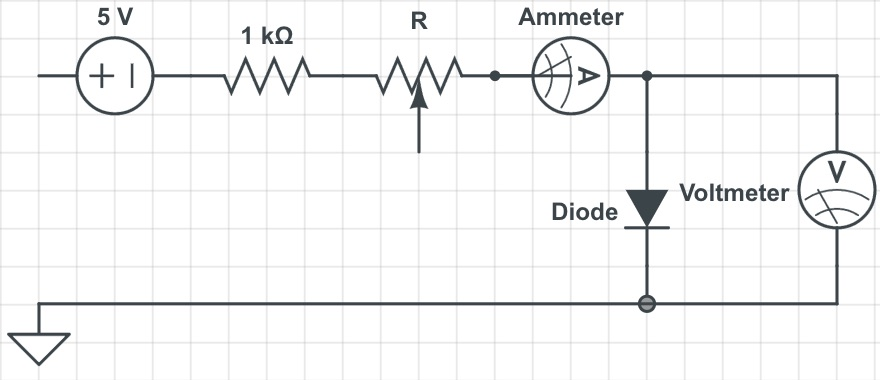
\includegraphics[scale=0.3]{lab1_diode1}\\			
		Figure 3: Ciruict Diagram with diode
	\end{center}
	We took some date points of V and I, then plotted the I-V curve.
	\begin{center} 
		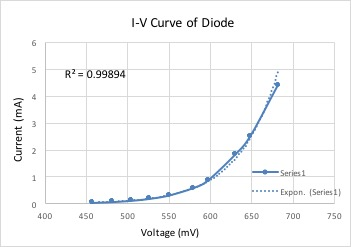
\includegraphics[scale=0.7]{lab1_diode2}\\			
		Figure 4: Non-ohmic IV curve of diode and its log-lin fit line
	\end{center}
	The curve displays a non-ohmic behavior. The logarithm fit line works well with the plot. So we can say the the voltage drop across the diode goes exponentially with the current. 
	\paragraph{ (j)}
	When a full 5V was put across the diode, the Ammeter read 0.998A, smoke came out and the diode was burned. The power supply also dropped to 1.764V to protect the instrument. 
	
\subsection*{Voltage Divider and Thevenin Mode}	
	\paragraph{ (k)}
	We measured the open cirucit voltage, $V_{R1} =V_{R2} =7.42V$,as the two resistors are connected in parrallel. Then we connected a 10k$\Omega$ load to the circuit as shown below. 
		\begin{center} 
			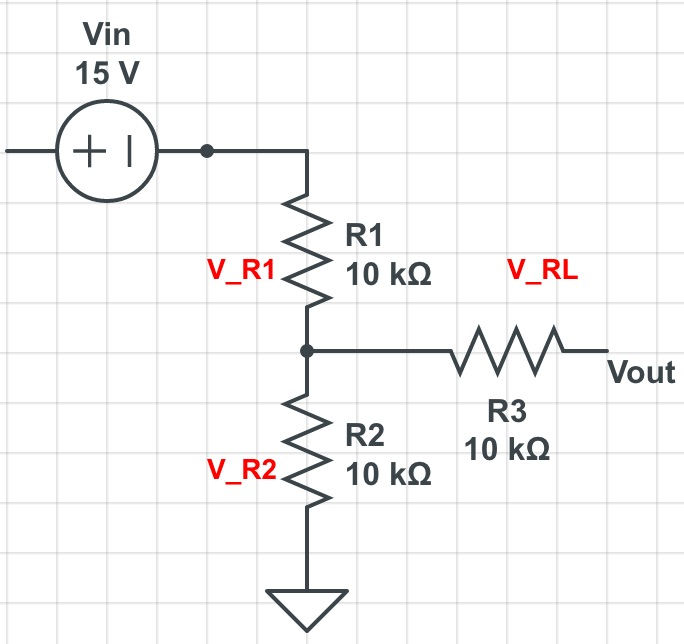
\includegraphics[scale=0.2]{lab1_k2}\\
			Figure 5: Voltage divider with load		
		\end{center}
	With the load, $V_{out}$ dropped from 7.42V to 4.70V. We measured $V_{R1}=7.42V, V_{R2}=V_{RL}=4.70V$. Because the current goes through $R_{1}$, and then branches out to $R_{2}$ and $R_{3}$ as they are in parrallel. \\
	Removing the load, we used Ammeter to measure the shortcircuit current $I_{ss}$ to be 1.51mA. It's safe to "short circuit" $V_{out}$ because the Ammeter shown in Fig.6 is in connected in series with $R_{1}$.
	\begin{center} 
		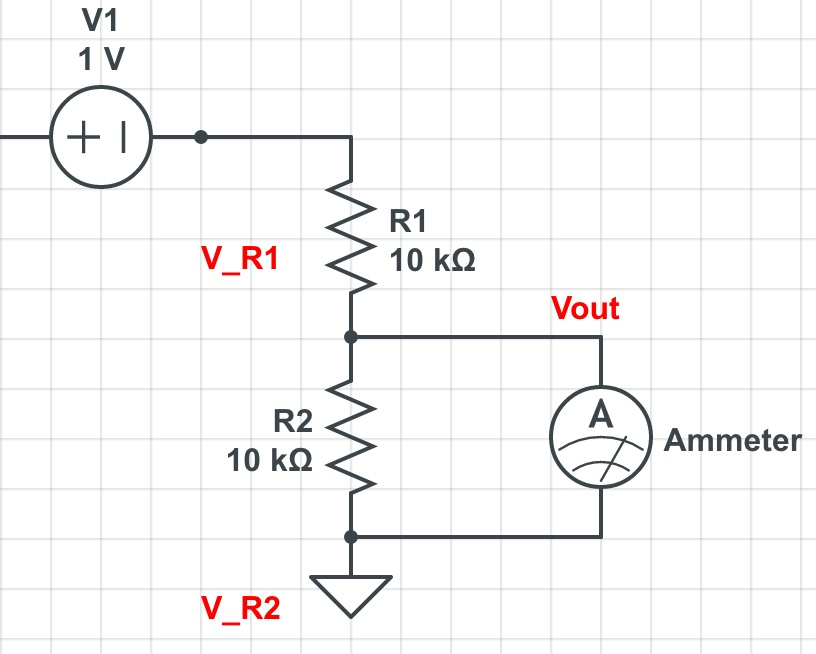
\includegraphics[scale=0.2]{lab1_thev2}\\			
		Figure 6: Voltage Divider without load 
	\end{center}
	The Thevenin equivalent circuit without $R_{load}$ is:
	\begin{center} 
		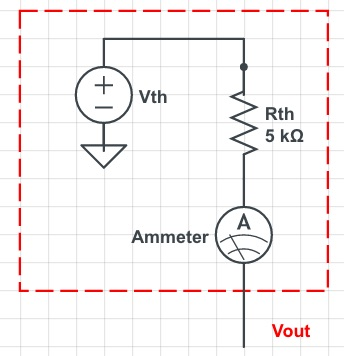
\includegraphics[scale=0.4]{lab1_thev4}\\			
		Figure 7: Thevenin equivalent without load
		\end{center}
	Where $V_{th}=V_{out}=7.5V$ which is close to the $V_{out}=7.42V$ before. Since $R_{th}=\frac{R_{1}R_{2}}{R_{1}+R_{2}}=\frac{100(k\Omega)^2}{20k\Omega}=5k\Omega$. So $I_{ss}=\frac{V_{th}}{R_{th}}=\frac{7.5V}{5000\Omega}=1.5mA$, which is about the same as the $I_{ss}=$1.51mA before in the original circuit.\\
	Adding a 10k$\Omega$ load, we have: 
	\begin{center} 
		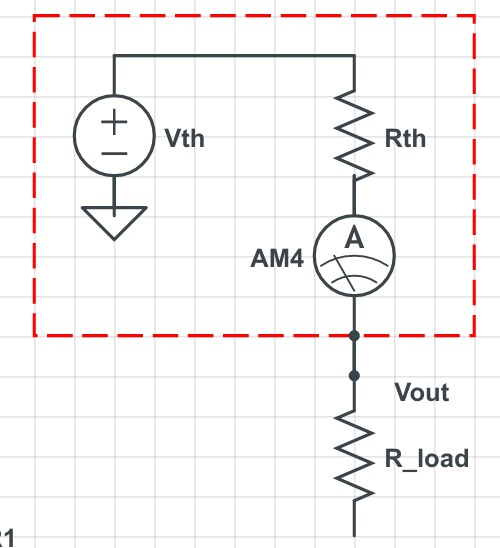
\includegraphics[scale=0.3]{lab1_thev3}\\			
		Figure 8: Thevenin equivalent with load
	\end{center}
The measured voltage $V_{out}=5.00V$, which is abou the same as the $V_{out}=4.70V$ in the first circuit.
\subsection*{Function generator}	
	\paragraph{ (l)}
	We used the sweep function of the function generator to go from a low start frequency to a high stop frequency, making an interesting "alarm" sound.
\subsection*{Oscilloscope}	
	\paragraph{ (m)}
	(1) We don't want to use auto trigger because it will automatically force the trigger to sweep even when there's no signal. In normal mode, the scope sweeps only when it's triggered by an input signal. We used auto trigger in part (a) because we just wanted to see the voltage on scope, and since we weren't sure about our signal so it'd hard to use normal trigger.  \\
	(2) We saw the risetime and falltime for square waves are not instantanous and not sharp. There's some noise osciallting at the edge. Risetime measurement on the scope measures the time it takes to go from, typically 10\% of a signal to 90\% (where 0\% is the lowest singal amplitude, 100\% is the highest). Similarly, falltime is the time going from 90\% to 10\%. The risetime/falltime here is not exactly the RC time constant but related to the time constant proportionally.\\ 
	(3) The better signal to trigger the square waves on the scope is to trigger on "edge", since square waves have clear edges.\\
	(4) AC coupling on the scope will take out the DC portion of the wave. So,when we looked at a low frequency such as 50 Hz on the ocilloscope with AC coupling, the low frequency part of the waves was cut off, as demonstrated below:
		\begin{center} 
			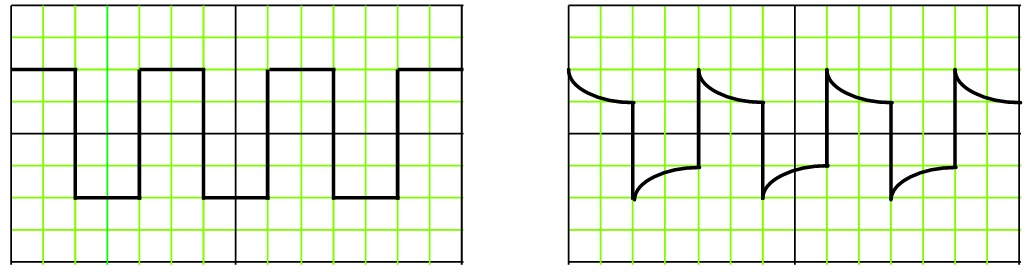
\includegraphics[scale=0.3]{lab1_accoupling}\\			
			Figure 9: DC (left) and AC (right) coupling on low-frequency\\
			(image source: http://slideplayer.com/slide/8551807/)
		\end{center}

	
\subsection*{AC Voltage Divider}	
	\paragraph{ (n)}
With the sine wave, the voltage divider works pretty much like the voltage divider without load in part (k). The measured votlage $V_{out}$ to the ground is about 6.5V, which is close to the 7.2V we got for the DC voltage divider.
\begin{center}
	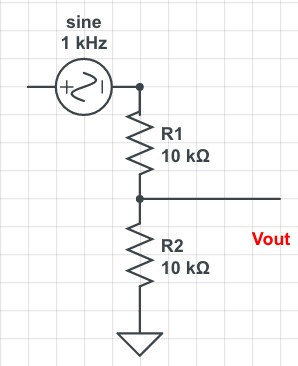
\includegraphics[scale=0.35]{lab1_ac}\\			
	Figure 10: AC voltage divider without load
\end{center}

	

\end{document}
